\apendice{Especificación de Requisitos}
\label{apendice:requisitos}

\section{Introducción}
En este anexo se detallan los requisitos que debe cumplir el sistema desarrollado en este Trabajo de Fin de Grado. Se presentarán los objetivos generales del proyecto, un catálogo de requisitos funcionales y no funcionales que definen el comportamiento y las cualidades de la infraestructura, los actores que interactúan con el sistema y los principales casos de uso.

\section{Objetivos Generales del Proyecto}
Como se detalló en el Capítulo 2, el objetivo principal de este TFG es el \textbf{diseño e implementación de una infraestructura de backend robusta, escalable y tolerante a fallos} para un sistema de procesamiento de vídeo. El propósito es crear una base sólida que permita la captura, transporte y análisis de sesiones de telerehabilitación, superando las limitaciones del sistema predecesor.

\section{Catálogo de Requisitos}
A continuación, se presenta un catálogo detallado de los requisitos que debe satisfacer el sistema.

\subsection{Requisitos Técnicos del Entorno}
Para la correcta ejecución y despliegue del sistema desarrollado, se deben cumplir una serie de requisitos tanto a nivel de hardware como de software en la máquina anfitriona (\textit{host}).

\subsubsection{Requisitos de Hardware}
Los requisitos de \textit{hardware} se refieren a la máquina física o virtual sobre la que se desplegará toda la infraestructura Docker.
\begin{itemize}
    \item \textbf{CPU:} Se recomienda un procesador multi-núcleo (4 o más núcleos) con soporte para tecnologías de virtualización (VT-x/AMD-V) habilitado en la BIOS/UEFI.
    \item \textbf{Memoria RAM:} Debido a la cantidad de servicios que se ejecutan simultáneamente (Jitsi, Kafka, Spark, etc.), se recomienda un mínimo de \textbf{16 GB de RAM} para un funcionamiento fluido.
    \item \textbf{Almacenamiento:} Se requiere un mínimo de 50 GB de espacio en disco disponible para el sistema operativo, las imágenes Docker y el almacenamiento de los vídeos generados. Es recomendable utilizar una unidad de estado sólido (SSD) para un mejor rendimiento.
    \item \textbf{Red:} Una conexión a internet estable y un \textit{router} con capacidad para configurar la re-dirección de puertos (\textit{port forwarding}), necesario para el despliegue de Jitsi con acceso externo.
\end{itemize}

\subsubsection{Requisitos de Software (Sistema Anfitrión)}
Estos son los componentes de software que deben estar instalados directamente en el sistema operativo anfitrión.
\begin{enumerate}
    \item \textbf{Sistema Operativo:} Se recomienda una distribución de Linux estable. Todo el desarrollo y las pruebas se han realizado sobre \textbf{Debian 12 "Bookworm"}.
    \item \textbf{Motor de Contenerización:}
    \begin{itemize}
        \item \textbf{Docker Engine:} Versión 20.10 o superior.
        \item \textbf{Docker Compose:} Versión v2.0 o superior (integrado como plugin de Docker).
    \end{itemize}
\end{enumerate}

\subsubsection{Requisitos de Software (Gestionados por Docker)}
Gracias a la contenerización, la mayoría de las dependencias de software están encapsuladas en sus respectivas imágenes Docker, eliminando la necesidad de instalarlas manualmente en el sistema anfitrión. Las imágenes y librerías principales son:
\begin{itemize}
    \item \textbf{Imágenes Docker Base:}
    \begin{itemize}
        \item \textit{Jitsi Meet Stack:} Imágenes oficiales del proyecto \texttt{docker-jitsi-meet} (jitsi/web, jitsi/prosody, jitsi/jicofo, jitsi/jvb, jitsi/jibri).
        \item \textit{Apache Kafka:} Imagen de Confluent Inc. (\texttt{confluentinc/cp-kafka}).
        \item \textit{Apache Spark:} Imagen de Bitnami (\texttt{bitnami/spark}) con un master y un worker.
        \item \textit{Python:} Imagen oficial de Python (\texttt{python:3.9-slim}) como base para el contenedor de procesamiento.
    \end{itemize}
    \item \textbf{Librerías de Python (instaladas vía \texttt{requirements.txt}):}
    \begin{itemize}
        \item \textit{pyspark}: para la interacción con el clúster de Spark.
        \item \textit{kafka-python}: para la comunicación con el broker de Kafka.
        \item \textit{numpy==1.26.4}: versión fijada para garantizar la compatibilidad con OpenCV.
        \item \textit{opencv-python}: para el procesamiento de los fotogramas de vídeo.
    \end{itemize}
\end{itemize}

\subsection{Requisitos Funcionales (RF)}
Los requisitos funcionales describen las capacidades y el comportamiento específico que la infraestructura debe ofrecer.

\begin{itemize}
    \item \textbf{RF-01: Captura de Sesiones de Vídeo.} El sistema debe ser capaz de grabar una sesión de videoconferencia completa, incluyendo audio y vídeo, y almacenarla como un archivo en formato MP4 en un directorio persistente.
    
    \item \textbf{RF-02: Detección de Nuevos Vídeos.} El sistema de procesamiento debe ser capaz de detectar automáticamente la presencia de nuevos archivos de vídeo en el directorio de entrada.
    
    \item \textbf{RF-03: Procesamiento de Vídeo.} El sistema debe leer un archivo de vídeo de entrada y aplicar sobre él una transformación de procesamiento de imágenes predefinida (ej. inversión de color) a cada fotograma.
    
    \item \textbf{RF-04: Almacenamiento de Resultados.} El sistema debe guardar el vídeo resultante del procesamiento como un nuevo archivo MP4 en un directorio de salida específico.
    
    \item \textbf{RF-05: Archivado de Vídeos Procesados.} Una vez que un vídeo ha sido procesado con éxito, el sistema debe mover el archivo original a un directorio de archivado para evitar su re procesamiento.
    
    \item \textbf{RF-06: Gestión de Servicios Orquestada.} Todos los componentes de la infraestructura (servicios de captura, bus de mensajería, clúster de procesamiento) deben poder ser desplegados y gestionados de forma conjunta mediante un único comando.
\end{itemize}

\subsection{Requisitos No Funcionales (RNF)}
Los requisitos no funcionales definen las cualidades del sistema y las restricciones bajo las cuales debe operar. Son especialmente críticos en un proyecto de infraestructura como este.

\begin{itemize}
    \item \textbf{RNF-01: Portabilidad.} La infraestructura completa debe ser portable entre diferentes máquinas de desarrollo o servidores, garantizando un comportamiento idéntico gracias al uso de contenedores Docker.
    
    \item \textbf{RNF-02: Escalabilidad.} La arquitectura debe estar diseñada para ser escalable. Esto implica que componentes como los nodos de procesamiento o los brokers de mensajería deben poder replicarse para manejar una mayor carga de trabajo en el futuro.
    
    \item \textbf{RNF-03: Fiabilidad.} El sistema debe ser fiable. El uso de un bus de mensajería debe garantizar que los datos no se pierdan durante el transporte entre los distintos componentes del pipeline.
    
    \item \textbf{RNF-04: Mantenibilidad.} El código fuente y la estructura de directorios deben estar organizados de forma clara y modular para facilitar su comprensión y futuras modificaciones.
    
    \item \textbf{RNF-05: Código Abierto.} Todos los componentes de software utilizados deben tener licencias de código abierto que permitan su uso y modificación en el marco de un proyecto académico.
\end{itemize}

\section{Actores del Sistema}
\label{sec:actores}
Aunque gran parte de este proyecto se centra en la infraestructura de \textit{backend}, el sistema completo está diseñado para ser utilizado por diferentes tipos de actores, cada uno con un rol específico.

\begin{enumerate}
    \item \emph{Paciente:} Es el usuario final del sistema de tele-rehabilitación. Su única función es unirse a la sesión de videoconferencia para realizar sus ejercicios.
    \item \emph{Terapeuta:} Es el profesional sanitario que dirige la sesión. Además de guiar al paciente, tiene la capacidad de iniciar y detener la grabación de la sesión de ejercicios.
    \item \emph{Administrador del Sistema:} Es el usuario técnico responsable de desplegar, gestionar y supervisar la infraestructura. Aunque no participa en la sesión, es quien asegura que el sistema esté operativo y quien podría acceder a los resultados del procesamiento para su validación.
\end{enumerate}

\begin{figure}[H]
    \centering
    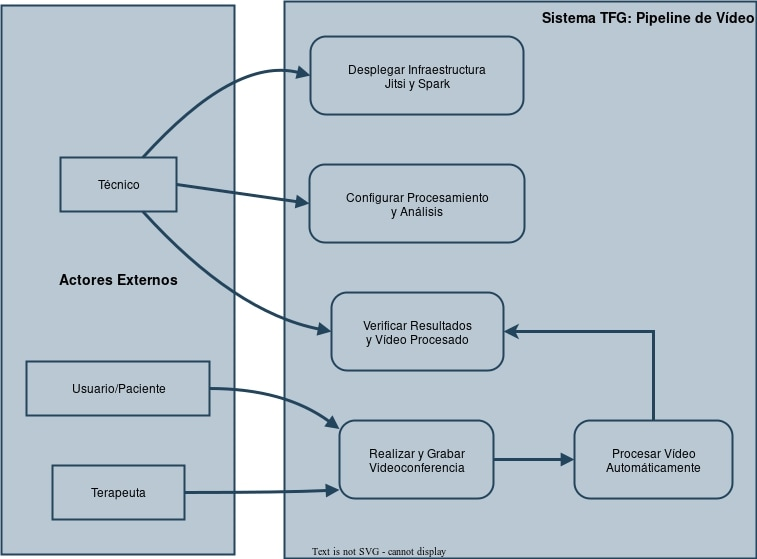
\includegraphics[width=0.8\textwidth]{img/Diagramacasodeuso.jpg}
    \caption{Diagrama de los principales casos de uso del sistema.}
    \label{fig:anexob_actores}
\end{figure}

\section{Catálogo de Requisitos Funcionales}
\label{sec:requisitos_funcionales}
A continuación, se detallan los requisitos funcionales del sistema, descritos como un flujo de trabajo lógico desde la perspectiva de los actores.

\begin{itemize}
	\item \textbf{RF.1: Realización de una Sesión de Telerehabilitación}
	\begin{itemize}
	    \item \textbf{RF.1.1:} El Paciente debe poder unirse a una sala de videoconferencia de Jitsi a través de un enlace web.
	    \item \textbf{RF.1.2:} El Terapeuta debe poder unirse a la misma sala de videoconferencia para dirigir la sesión.
	\end{itemize}
	
	\item \textbf{RF.2: Gestión de la Grabación de la Sesión}
	\begin{itemize}
	    \item \textbf{RF.2.1:} El Terapeuta debe disponer de un botón o función en la interfaz de Jitsi para iniciar la grabación de la sesión.
	    \item \textbf{RF.2.2:} Al iniciar la grabación, el sistema debe activar automáticamente el servicio Jibri, que se unirá a la llamada como un participante silencioso.
	    \item \textbf{RF.2.3:} El Terapeuta debe poder detener la grabación en cualquier momento.
        \item \textbf{RF.2.4:} Al detener la grabación, el sistema debe guardar la sesión completa como un único archivo de vídeo en formato MP4 en un directorio de entrada predefinido en el servidor.
	\end{itemize}
	
	\item \textbf{RF.3: Procesamiento Automático del Vídeo Grabado}
	\begin{itemize}
	    \item \textbf{RF.3.1:} El sistema debe detectar automáticamente cuándo un nuevo fichero MP4 ha sido depositado en el directorio de entrada.
	    \item \textbf{RF.3.2:} El sistema debe iniciar un proceso que tome el nuevo vídeo y lo envíe a través del pipeline de datos.
	    \item \textbf{RF.3.3:} El pipeline debe aplicar una transformación de vídeo predefinida (la prueba de concepto de inversión de color) a todos los fotogramas del vídeo.
	    \item \textbf{RF.3.4:} El sistema debe guardar el vídeo resultante de la transformación en un directorio de salida.
	\end{itemize}
	
	\item \textbf{RF.4: Gestión de Ficheros y Resultados}
	\begin{itemize}
	    \item \textbf{RF.4.1:} El Administrador del Sistema debe poder acceder al directorio de salida para verificar el vídeo procesado.
	    \item \textbf{RF.4.2:} Una vez que un vídeo original ha sido procesado con éxito, el sistema debe moverlo automáticamente a una carpeta de archivado para evitar que sea procesado de nuevo.
	\end{itemize}
\end{itemize}

\section{Casos de Uso}
A continuación, se describen los principales casos de uso desde la perspectiva del Administrador del Sistema.

\subsection{Caso de Uso 1: Desplegar la Infraestructura Completa}
\begin{itemize}
    \item \textbf{Actor:} Administrador del Sistema.
    \item \textbf{Descripción:} El administrador despliega todos los servicios de la arquitectura (Jitsi, Kafka, Spark, etc.) en un entorno limpio.
    \item \textbf{Precondiciones:} El sistema anfitrión (Debian 12) tiene Docker y Docker Compose instalados.
    \item \textbf{Flujo Principal:}
        \begin{enumerate}
            \item El administrador clona el repositorio del proyecto desde GitHub.
            \item El administrador configura los ficheros \texttt{.env} necesarios.
            \item El administrador ejecuta el comando \texttt{docker-compose up} principal.
            \item El sistema levanta todos los contenedores, crea las redes y los volúmenes necesarios.
        \end{enumerate}
    \item \textbf{Postcondiciones:} Todos los servicios están en ejecución y listos para operar.
\end{itemize}

\subsection{Caso de Uso 2: Ejecutar el Pipeline de Procesamiento de Vídeo}
\begin{itemize}
    \item \textbf{Actor:} Administrador del Sistema (o un proceso automatizado).
    \item \textbf{Descripción:} El administrador inicia el script que procesa un vídeo grabado previamente.
    \item \textbf{Precondiciones:} La infraestructura está desplegada y en ejecución. Existe al menos un archivo MP4 en el directorio de entrada.
    \item \textbf{Flujo Principal:}
        \begin{enumerate}
            \item El administrador ejecuta el script de procesamiento de vídeo.
            \item El script detecta el vídeo más antiguo en la carpeta de entrada.
            \item Los datos del vídeo se envían a través de Kafka y son procesados por Spark.
            \item Se genera un nuevo archivo de vídeo procesado en el directorio de salida.
            \item El archivo de vídeo original se mueve al directorio de archivado.
        \end{enumerate}
    \item \textbf{Postcondiciones:} El vídeo ha sido procesado y archivado. El sistema queda a la espera de nuevos vídeos.
\end{itemize}

\section{Especificación de requisitos}
En este apartado se van a mostrar, por una parte el diagrama de caso de uso, como se puede observar en las figuras  \ref{f:casoUso} y por otra, las tablas de casos de uso.


\begin{figure}[H]
 \centering
\subfloat{
    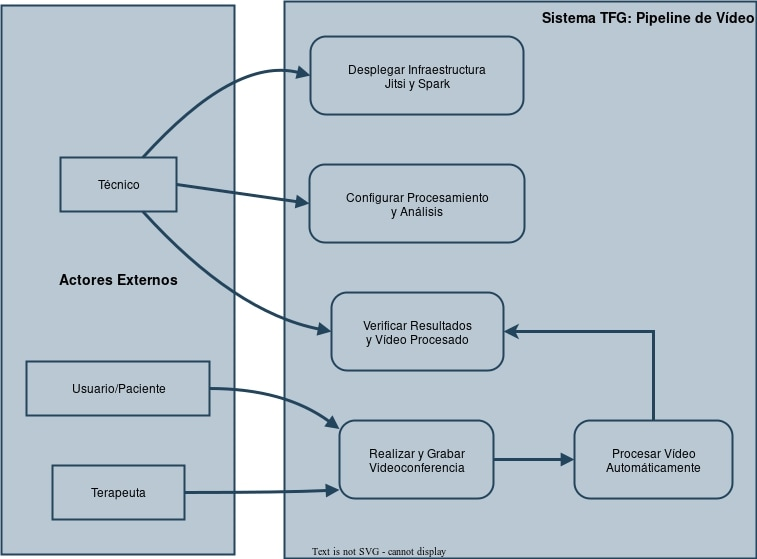
\includegraphics[width=\textwidth]{img/Diagramacasodeuso.jpg}}
 \caption{Diagrama de casos de uso.}
 \label{f:casoUso}
\end{figure}


% --- CASO DE USO 1 ---
\begin{table}[H]
    \centering
    \caption{Caso de uso 1: Desplegar la Infraestructura Completa.}
    \label{tab:uc1}
    \begin{tabular}{|p{3cm}|p{0.75cm}|p{8.5cm}|}
        \hline
        \textbf{Descripción} & \multicolumn{2}{p{9.25cm}|}{Permite al Administrador del Sistema desplegar todos los servicios de la arquitectura de forma orquestada.} \\
        \hline
        \multirow{3}{3cm}{\textbf{Requisitos}} & \multicolumn{2}{p{9.25cm}|}{RF.1.1} \\ \cline{2-3}
         & \multicolumn{2}{p{9.25cm}|}{RF.1.2} \\ \cline{2-3}
         & \multicolumn{2}{p{9.25cm}|}{RF.1.3} \\
        \hline
        \textbf{Precondiciones} & \multicolumn{2}{p{9.25cm}|}{El sistema anfitrión (Debian 12) tiene Docker y Docker Compose instalados y funcionando correctamente.} \\
        \hline
        \multirow{4}{3cm}{\textbf{Secuencia Normal}} & \textbf{Paso} & \textbf{Acción} \\ \cline{2-3}
         & 1 & El Administrador clona el repositorio del proyecto desde GitHub. \\ \cline{2-3}
         & 2 & El Administrador configura los ficheros de entorno (\texttt{.env}) necesarios. \\ \cline{2-3}
         & 3 & El Administrador ejecuta el comando \texttt{docker-compose up} desde la raíz del proyecto. \\ \cline{2-3}
         & 4 & El sistema levanta todos los contenedores, crea las redes y los volúmenes necesarios. \\
        \hline
        \textbf{Postcondiciones} & \multicolumn{2}{p{9.25cm}|}{Todos los servicios de la infraestructura (Jitsi, Kafka, Spark) están en ejecución y listos para operar.} \\
        \hline
        \textbf{Excepciones} & \multicolumn{2}{p{9.25cm}|}{El host no tiene conexión a internet, lo que impide la descarga de las imágenes Docker desde los registros públicos.} \\
        \hline
        \textbf{Importancia} & \multicolumn{2}{p{9.25cm}|}{Alta} \\
        \hline
        \textbf{Urgencia} & \multicolumn{2}{p{9.25cm}|}{Alta} \\
        \hline
    \end{tabular}
\end{table}

% --- CASO DE USO 2 ---
\begin{table}[H]
    \centering
    \caption{Caso de uso 2: Ejecutar el Pipeline de Procesamiento de Vídeo.}
    \label{tab:uc2}
    \begin{tabular}{|p{3cm}|p{0.75cm}|p{8.5cm}|}
        \hline
        \textbf{Descripción} & \multicolumn{2}{p{9.25cm}|}{Permite procesar un vídeo grabado en una sesión de Jitsi para obtener un resultado analizado.} \\
        \hline
        \multirow{4}{3cm}{\textbf{Requisitos}} & \multicolumn{2}{p{9.25cm}|}{RF.2.1, RF.2.2, RF.3.1, RF.3.2, RF.3.3, RF.4.1, RF.4.2, RF.4.3} \\
        \hline
        \textbf{Precondiciones} & \multicolumn{2}{p{9.25cm}|}{La infraestructura está desplegada y en ejecución. Se ha realizado una sesión de telerehabilitación y el archivo MP4 resultante se encuentra en el directorio de entrada.} \\
        \hline
        \multirow{4}{3cm}{\textbf{Secuencia Normal}} & \textbf{Paso} & \textbf{Acción} \\ \cline{2-3}
         & 1 & El Terapeuta inicia y finaliza la grabación de una sesión en Jitsi. Jibri guarda el fichero MP4. \\ \cline{2-3}
         & 2 & El Administrador (o un proceso automatizado) ejecuta el script de procesamiento. \\ \cline{2-3}
         & 3 & El script detecta el vídeo, lo procesa a través del pipeline Kafka/Spark y guarda el resultado. \\ \cline{2-3}
         & 4 & El script archiva el vídeo original para evitar su reprocesamiento. \\
        \hline
        \textbf{Postcondiciones} & \multicolumn{2}{p{9.25cm}|}{El vídeo ha sido procesado y el resultado se encuentra en el directorio de salida. El vídeo original ha sido archivado.} \\
        \hline
        \textbf{Excepciones} & \multicolumn{2}{p{9.25cm}|}{No hay vídeos nuevos en el directorio de entrada; el script finaliza sin realizar ninguna acción.} \\
        \hline
        \textbf{Importancia} & \multicolumn{2}{p{9.25cm}|}{Alta} \\
        \hline
        \textbf{Urgencia} & \multicolumn{2}{p{9.25cm}|}{Alta} \\
        \hline
    \end{tabular}
\end{table}